\chapter{Analisis dan Perancangan}

\section{Analisis Masalah}\label{section-problem-analysis}

Akan digunakan teknik parametrik neural untuk membangkitkan suara alat musik gesek. Hal ini karena penggabungan komponen-komponen CSEMP alat musik gesek yang ada tidak memungkinkan karena masalah kompatibilitas. Selain itu, terdapat beberapa kemiripan dengan penerapan teknik parametrik neural untuk sintesis suara nyanyian dari sisi kontinuitas eksitasi dan jumlah not pada satu waktu. Teknik neural parametrik juga lebih baik dari sisi waktu eksekusi dibandingkan dengan teknik pembangkitan \textit{waveform} secara langsung. Untuk teknik neural parametrik ini, terdapat beberapa perbedaan masalah dengan penelitian sebelumnya\parencite{bonada2017singing}. Perbedaan masalah yang terjadi terdapat pada karakteristik suara alat musik, data input untuk sintesis, \textit{timing}. Perbedaan masalah-masalah ini adalah:

\begin{enumerate}

\item Perbedaan karakteristik suara alat musik gesek dan suara nyanyian terletak pada gaung. Suara nyanyian memiliki gaung yang sedikit, sehingga tidak terdapat polifoni yang signifikan. Pada alat musik gesek, gaung sangat banyak digunakan sebagai bentuk ekspresi, sehingga terjadi polifoni akibat gaung.

\item \textit{Timing} not dalam alat musik gesek memiliki karakteristik yang berbeda dengan suara nyanyian. Dalam sistem \textit{baseline} untuk suara nyanyian, terdapat \textit{timing} fonetik. Dalam sistem ini, tidak ada \textit{timing} fonetik. Hanya dibutuhkan \textit{timing} not saja.

\item Perbedaan masalah untuk data input sintesis terkait dengan \textit{timbre}. Dalam pembangkitan suara alat musik gesek, \textit{timbre} ditentukan oleh konteks. Hal ini berbeda dengan penelitian sebelumnya, di mana \textit{timbre} ditentukan dari rangkaian fonem yang terdapat dalam data input.

\end{enumerate}

\section{Rancangan Umum Sistem}

Arsitektur sistem perbaikan terlihat pada gambar \ref{fig-system-overview}, sebagai modifikasi dari gambar \ref{fig-system-overview-bonada}. \ref{tab-models-in-out} Untuk menerapkan sistem yang dijelaskan pada subbab \ref{literature-neural-parametric} ke alat musik gesek agar dapat dijalankan dan menghasilkan suara alat musik gesek, Dilakukan beberapa penyesuaian agar masalah-masalah pada subbab \ref{section-problem-analysis} dapat diatasi:

\begin{enumerate}

    \item Perbedaan karakteristik suara alat musik diatasi dengan mengganti vocoder dengan teknik kompresi audio yang sesuai dengan alat musik gesek
    \item Aspek fonetik ditiadakan dari data \textit{timing} dan masukan kontrol untuk model \textit{timbre}
    \item Agar penentuan \textit{timbre} mempertimbangkan konteks, masukan model \textit{timbre} ditambahkan dengan masukan partitur dan \textit{timing} not

\end{enumerate}

Dalam sistem ini, pengkodean dan sintesis suara audio tidak digunakan dengan vocoder. Pengkodean dan sintesis suara audio dilakukan dengan pengkodean harmonik terarah plus stokastik dan sintesis harmonik plus stokastik. Teknik ini diharapkan mampu mengatasi adanya gaung.

Dalam sistem ini, seperti pada sistem pembangkit nyanyian, memiliki tiga model yang dilatih dengan data latih. Model-model itu adalah model \textit{timing}, model \textit{pitch}, dan model \textit{timbre}. Masukan dan keluaran setiap model tertulis pada tabel \ref{tab-models-in-out}

Model \textit{timing} dalam sistem ini dilatih menggunakan partitur dan \textit{timing} not. Dengan demikian, diharapkan model \textit{timing} dapat memprediksi \textit{timing} dari not dalam partitur.

Model \textit{pitch} dalam sistem ini dilatih untuk menghasilkan F0. Masukan model ini adalah partitur dan \textit{timing}. Dalam pelatihan, masukan partitur dan \textit{timing} not diambil dari data latih, dan parameter vocoder diambil dari hasil pengkodean harmonik terarah plus stokastik terhadap audio.

\begin{figure}[h]
    \centering
    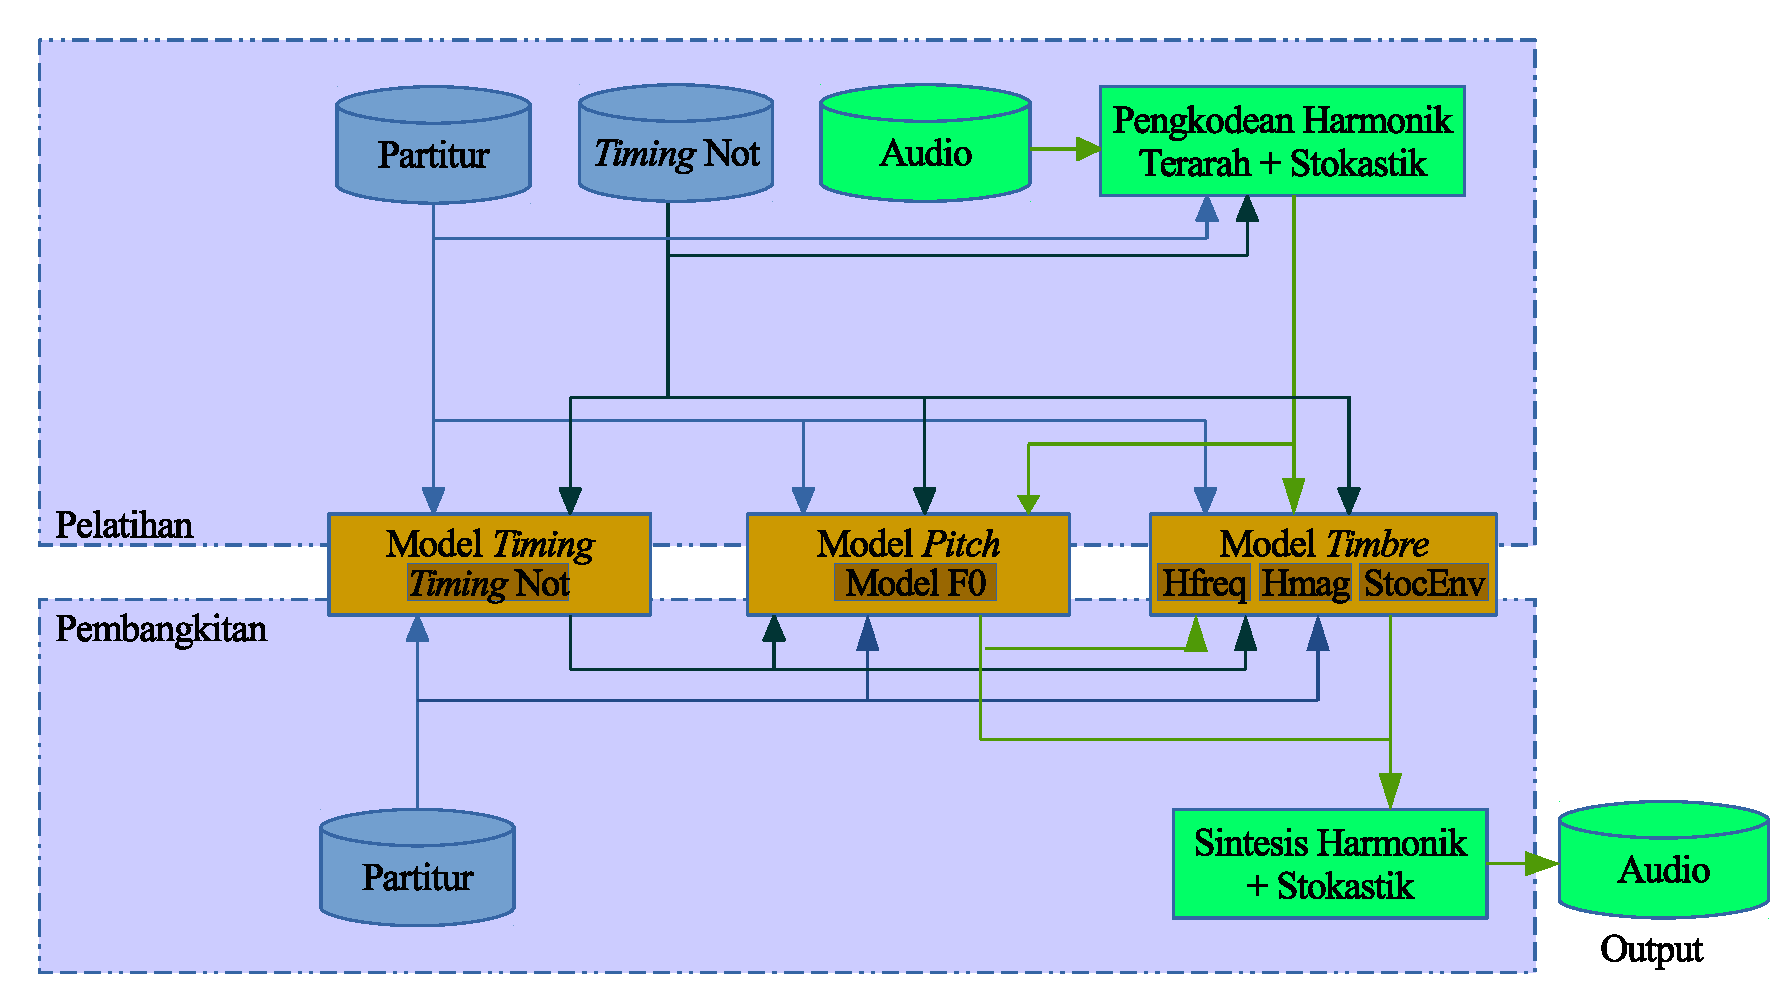
\includegraphics[width=0.8\textwidth]{resources/system-overview.eps}
    \caption{Adopsi teknik neural parametrik untuk permainan musik ekspresif alat musik gesek (modifikasi gambar \ref{fig-system-overview-bonada})}\label{fig-system-overview}
\end{figure}

Pada tahap pembangkitan, sistem ini mampu menerima partitur dan menghasilkan audio. Keluaran perantara yang dihasilkan adalah parameter vocoder, yang kemudian digunakan oleh vocoder untuk menghasilkan audio.

Hal pertama yang dilakukan dalam tahap pembangkitan adalah prediksi \textit{timing} not. Setelah itu, partitur dan \textit{timing} not digunakan untuk memprediksi \textit{pitch} dan \textit{timbre}, dengan model yang sesuai. Parameter \textit{pitch} dan parameter \textit{timbre} digunakan untuk sintesis vocoder.

Tiap model dari model-model ini adalah model regresi. Untuk model \textit{timing}, digunakan jaringan syaraf tiruan \textit{feedforward}. Untuk model \textit{pitch} dan model \textit{timbre}, digunakan jaringan syaraf tiruan dengan konvolusi kausal terdilasi. Masukan dari jaringan syaraf tiruan ini terdiri dari masukan fitur akustik output waktu sebelumnya dan masukan kontrol.

Masukan kontrol jaringan syaraf tiruan ini berasal dari partitur dan dari \textit{timing}. Untuk model \textit{timing}, masukan kontrol hanya berasal dari partitur. Untuk model \textit{pitch} dan model \textit{timbre}, masukan kontrol berasal dari partitur dan berasal dari \textit{timing}.

Masukan dari partitur dapat menunjukkan kondisi sesaat dan konteks. Kondisi sesaat berupa \textit{pitch} asli, panjang not, dan waktu dalam not. Kondisi konteks dapat berupa not sebelum dan sesudah, interval, ataupun kondisi-kondisi lainnya hasil analisis karya. Namun, kakas analisis karya mungkin tidak akan digunakan karena riset terkait analisis karya menggunakan komputer masih minim.

\begin{table}[h]
    \centering
    \caption{Masukan dan Keluaran Tiap Model dalam Sistem Sintesis Parametrik Neural Suara Alat Musik Gesek }\label{tab-models-in-out}
    \begin{tabular}{ |c|c|c| } 
     \hline
     Model & Masukan & Keluaran \\
     \hline 
     Model \textit{timing} & partitur & \textit{timing} not  \\ 
     \hline
     Model \textit{pitch} & partitur & F0 \\ 
      & \textit{timing} not  & \\ 
     \hline
     Model \textit{timbre} & \textit{timing} not & Komponen harmonik \\ 
      & F0& Komponen aperiodisitas\\ 
     \hline
    \end{tabular}
\end{table}

\section{Pengkodean Harmonik Terarah Plus Stokastik}

Yang menyebabkan vocoder tidak dapat digunakan adalah penetapan frekuensi fundamental yang tidak menekankan not yang sedang berbunyi, serta penggunaan amplop spektral untuk merepresentasikan timbre. Dengan adanya gaung, terutama pada gaung yang lebih rendah daripada not yang sedang dibunyikan, vocoder akan banyak mendeteksi frekuensi fundamental gaung dan mengabaikan frekuensi fundamental not. Gaung pada spektrum-spektrum di luar frekuensi fundamental dan frekuensi harmonik juga akan mempengaruhi estimasi amplop spektral. Estimasi amplop spektral menggunakan asumsi bahwa suara dihasilkan dari gelombang glottal yang disaring dengan sebuah amplop spektral yang kontinu.

Agar penentuan frekuensi fundamental dari audio tidak dipengaruhi oleh gaung, pendeteksian frekuensi fundamental pada tiap langkah waktu dibatasi pada sekitar kemungkinan frekuensi fundamental not yang sedang dibunyikan pada langkah waktu tersebut. Untuk itu, diasumsikan bahwa frekuensi fundamental not yang sedang dibunyikan berada di sekitar frekuensi standar not dalam \textit{equal-temperament tuning}.

Pencarian frekuensi fundamental dilakukan dengan batas bawah dan batas atas yang bergantung pada not yang sedang dibunyikan (terarah oleh partitur dan \textit{timing not}). Batas bawah dan batas atas pencarian frekuensi fundamental terlihat pada pertidaksamaan \ref{eq-f0-bounds}. Di sini $note[t]$ adalah not yang dibunyikan pada waktu $t$. ${f_0}_{eq}(note[t])$ adalah frekuensi standar not $note[t]$ dalam \textit{equal-temperament tuning}. $f_0[t]$ adalah frekuensi fundamental sinyal suara pada waktu $t$. $pbt$ adalah \textit{threshold} deviasi \textit{pitch} dalam satuan \textit{semitone}.

\begin{equation}
    \dfrac{{f_0}_{eq}(note[t])}{2^{(pbt/12)}} \leq f_0[t] \leq 2^{(pbt/12)}{f_0}_{eq}(note[t])
\end{equation}\label{eq-f0-bounds}

Agar gaung tidak mempengaruhi estimasi timbre, asumsi gelombang glottal dan amplop spektral tidak digunakan. Suara alat musik gesek diasumsikan berupa kumpulan gelombang-gelombang sinusoidal pada frekuensi-frekuensi harmonik saja, dengan tiap harmonik memiliki kemungkinan pergeseran. Pada tiap langkah waktu, setelah ditemukan frekuensi fundamental pada langkah waktu tersebut, dilakukan estimasi frekuensi-frekuensi harmonik dan ukuran tiap harmonik. Adapun fase dari tiap gelombang harmonik diabaikan.

Sisa spektrum yang tidak dapat dikodekan dengan gelombang-gelombang sinusoidal pada tiap harmonik tersebut kemudian dikodekan dengan model stokastik. Model ini merepresentasikan aperiodisitas.

Dengan demikian, hasil pengkodean harmonik terarah plus stokastik memiliki format yang sama dengan pengkodean harmonik plus stokastik. Hasilnya berupa deskripsi frekuensi fundamental, frekuensi dan ukuran harmonik, dan stokastik untuk setiap langkah waktu. Yang membedakan keduanya adalah adanya batasan frekuensi fundamental yang diarahkan oleh data partitur dan \textit{timing not}

Pengkodean dengan cara ini mampu mengatasi polifoni yang diakibatkan oleh gaung. Polifoni yang diakibatkan karena dua atau lebih not berbunyi sekaligus tidak dapat diatasi dengan cara ini. Cara ini hanya mampu mengekstrak satu frekuensi fundamental dari setiap langkah waktu.

\section{Model \textit{Timing}}

Model \textit{timing} berfungsi menentukan panjang aktual dari tiap not. Panjang aktual dari tiap not ini kemudian digunakan untuk menentukan waktu-waktu pergantian satu not ke not berikutnya.

Model \textit{timing} dilatih dengan pasangan data latih fitur-fitur not dalam partitur dan \textit{timing} not tersebut. Sebuah jaringan syaraf tiruan \textit{feedforward} terhubung penuh digunakan untuk membangun model \textit{timing}. Keluaran yang diharapkan dari model ini adalah deviasi panjang not. Untuk tiap not, berikut ini adalah fitur-fitur not yang digunakan:

\begin{enumerate}
    \item panjang not yang tertulis dalam partitur
    \item panjang not sebelumnya yang tertulis dalam partitur
    \item posisi not dalam bar
    \item apakah not merupakan tanda istirahat
    \item apakah not sebelumnya merupakan tanda istirahat
\end{enumerate}

\section{Model \textit{Pitch}}

Model \textit{pitch} berfungsi membangkitkan frekuensi fundamental untuk tiap langkah waktu. Digunakan jaringan syaraf tiruan dengan arsitektur yang tampak pada gambar \ref{fig-network-architecture}.

\begin{figure}[h]
    \centering
    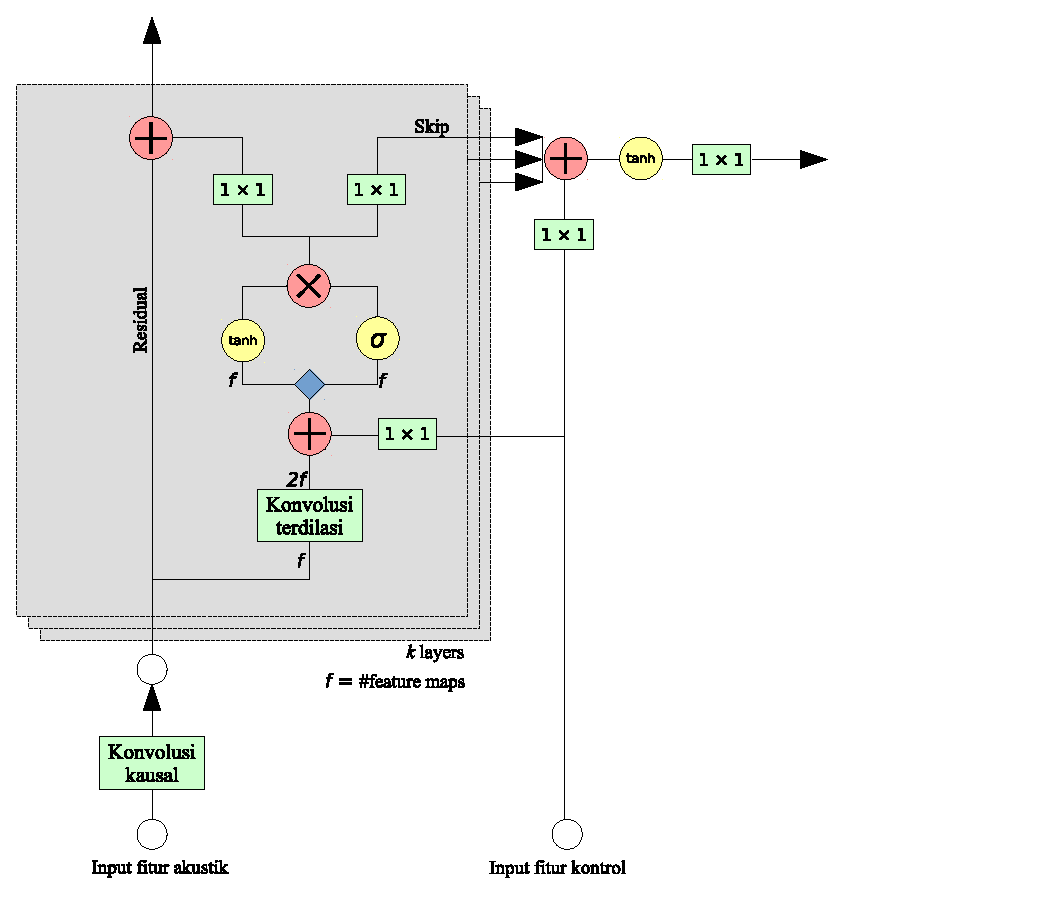
\includegraphics[width=0.8\textwidth]{resources/network-architecture.eps}
    \caption{Arsitektur jaringan syaraf tiruan modifikasi WaveNet yang digunakan pada sintesis neural parametrik untuk alat musik gesek (modifikasi dari gambar \ref{fig-network-architecture-bonada})}\label{fig-network-architecture}
\end{figure} 

Jaringan syaraf tiruan ini memiliki lapisan keluaran linear. Berbeda dengan sintesis nyanyian, distribusi keluaran dari jejaring ini belum diketahui. Karena keluaran linear merupakan keluaran paling sederhana untuk regresi, maka digunakan keluaran ini.

Input jaringan syaraf tiruan ini terdiri dari dua, yaitu input fitur akustik keluaran sebelumnya, dan input kontrol. Input kontrol berasal dari partitur.

Pembangkitan dilakukan untuk tiap langkah waktu secara berurutan dari depan ke belakang. Untuk tiap langkah waktu, keluaran dari beberapa langkah waktu sebelumnya, sepanjang medan reseptif, menjadi masukan pada langkah ini.

Fitur akustik yang dibangkitkan dan menjadi input fitur akustik berikutnya adalah deviasi f0, bukan f0 sebenarnya. Hal ini untuk menjaga konteks deviasi antar not. Deviasi f0 pada suatu not dipengaruhi oleh deviasi f0 pada not sebelumnya. Lebih lanjut, deviasi ini dihitung dalam skala logaritmik. Hubungan antara deviasi f0 dengan f0 ditunjukkan dalam persamaan \ref{f0-deviation}, dengan $\Delta_{f_0}[t]$ adalah deviasi f0. Pada tahap pembangkitan, f0 dihitung dari persamaan ini.

\begin{equation}
    \Delta_{f_0}[t] = ln(f_0[t]) - ln({f_0}_{eq}(note[t]))
\end{equation}\label{f0-deviation}

Input kontrol yang digunakan berasal dari partitur dan estimasi \textit{timing} keluaran model \textit{timing}. Berdasarkan keluaran model \textit{timing}, dapat diketahui not pada partitur yang dibunyikan pada satu langkah waktu. Berdasarkan not tersebut, input kontrol ini adalah sebagai berikut:

\begin{enumerate}
    \item \textit{pitch} $k$ not sebelumnya (one-hot posisi dalam oktaf dan nomor oktaf, relatif terhadap tanda kunci)
    \item \textit{pitch} not saat ini (one-hot posisi dalam oktaf dan nomor oktaf, relatif terhadap tanda kunci)
    \item \textit{pitch} $k$ not sesudahnya (one-hot posisi dalam oktaf dan nomor oktaf, relatif terhadap tanda kunci)
    \item tanda kunci
    \item durasi $k$ not sebelumnya
    \item durasi not saat ini
    \item durasi $k$ not sesudahnya
    \item posisi dalam not
\end{enumerate}

\section{Model \textit{Timbre}}

Model \textit{timbre} berfungsi membangkitkan representasi \textit{timbre}. Serupa dengan model \textit{pitch}, representasi \textit{timbre} untuk tiap langkah waktu dibangkitkan dengan input fitur akustik keluaran langkah-langkah waktu sebelumnya dan input kontrol. Digunakan jaringan syaraf tiruan dengan arsitektur pada gambar \ref{fig-network-architecture}.

Representasi \textit{timbre} yang menjadi keluaran dan input fitur akustik model ini adalah sebagai berikut:

\begin{enumerate}
    \item $ln(f_h)$: frekuensi harmonik ke-$h$ dalam skala logaritmik, untuk semua komponen harmonik
    \item $mag_h$: ukuran (desibel) komponen harmonik ke-$h$, untuk semua komponen harmonik
    \item $stoc_s$: ukuran komponen stokastik ke-$s$
\end{enumerate}

Frekuensi fundamental keluaran model \textit{pitch} juga menjadi masukan model \text{timbre}. Input kontrol untuk model ini adalah sebagai berikut:
\begin{enumerate}
    \item frekuensi fundamental ($f_0$)
    \item \textit{pitch} $k$ not sebelumnya (one-hot posisi dalam oktaf dan nomor oktaf, relatif terhadap tanda kunci)
    \item \textit{pitch} not saat ini (one-hot posisi dalam oktaf dan nomor oktaf, relatif terhadap tanda kunci)
    \item \textit{pitch} $k$ not sesudahnya (one-hot posisi dalam oktaf dan nomor oktaf, relatif terhadap tanda kunci)
    \item tanda kunci
    \item durasi $k$ not sebelumnya
    \item durasi not saat ini
    \item durasi $k$ not sesudahnya
    \item posisi dalam not
\end{enumerate}

\section{Data Partitur, \textit{Timing}, dan Audio}

Untuk melatih sistem ini, dibutuhkan data latih berupa partitur, \textit{timing} dan rekaman audio. Untuk itu, dibutuhkan partitur dan rekaman audio yang bersesuaian. Data dikumpulkan secara manual.

Partitur didapatkan dari Petrucci Music Library, dengan memilih secara berurutan dari daftar lagu untuk satu alat musik gesek. Dari daftar lagu tersebut, dipilih lagu yang dapat ditemukan rekaman audionya pada situs \textit{media sharing} publik.

Tidak semua lagu yang memiliki rekaman audio bersesuaian digunakan. Partitur dikumpulkan berurutan secara alfabetis dengan kriteria minimal total durasi 30 menit. Minimal total durasi ini didasarkan kepada riset neural parametrik nyanyian oleh Bonada.

Partitur terkumpul kemudian disalin dari format gambar atau PDF ke dalam format MIDI. Penyalinan ke dalam format MIDI dilakukan secara manual

Karena pengkodean harmonik plus sinusoidal hanya mampu menghasilkan suara monofonik, maka partitur dan rekaman tersebut kemudian dipotong-potong ke segmen-segmen yang monofonik. Segmen-segmen polifonik tidak digunakan.

Data \textit{timing} dibuat secara manual dari rekaman audio. Anotator mencatat waktu-waktu perubahan not dengan cara mendengarkan rekaman suara, dibantu dengan tampilan spektogram.